\part{蓝光二极管}

\section{2014年诺贝尔物理学奖}

\begin{slide}{\url{https://www.nobelprize.org/uploads/2018/06/press-25.pdf}}
  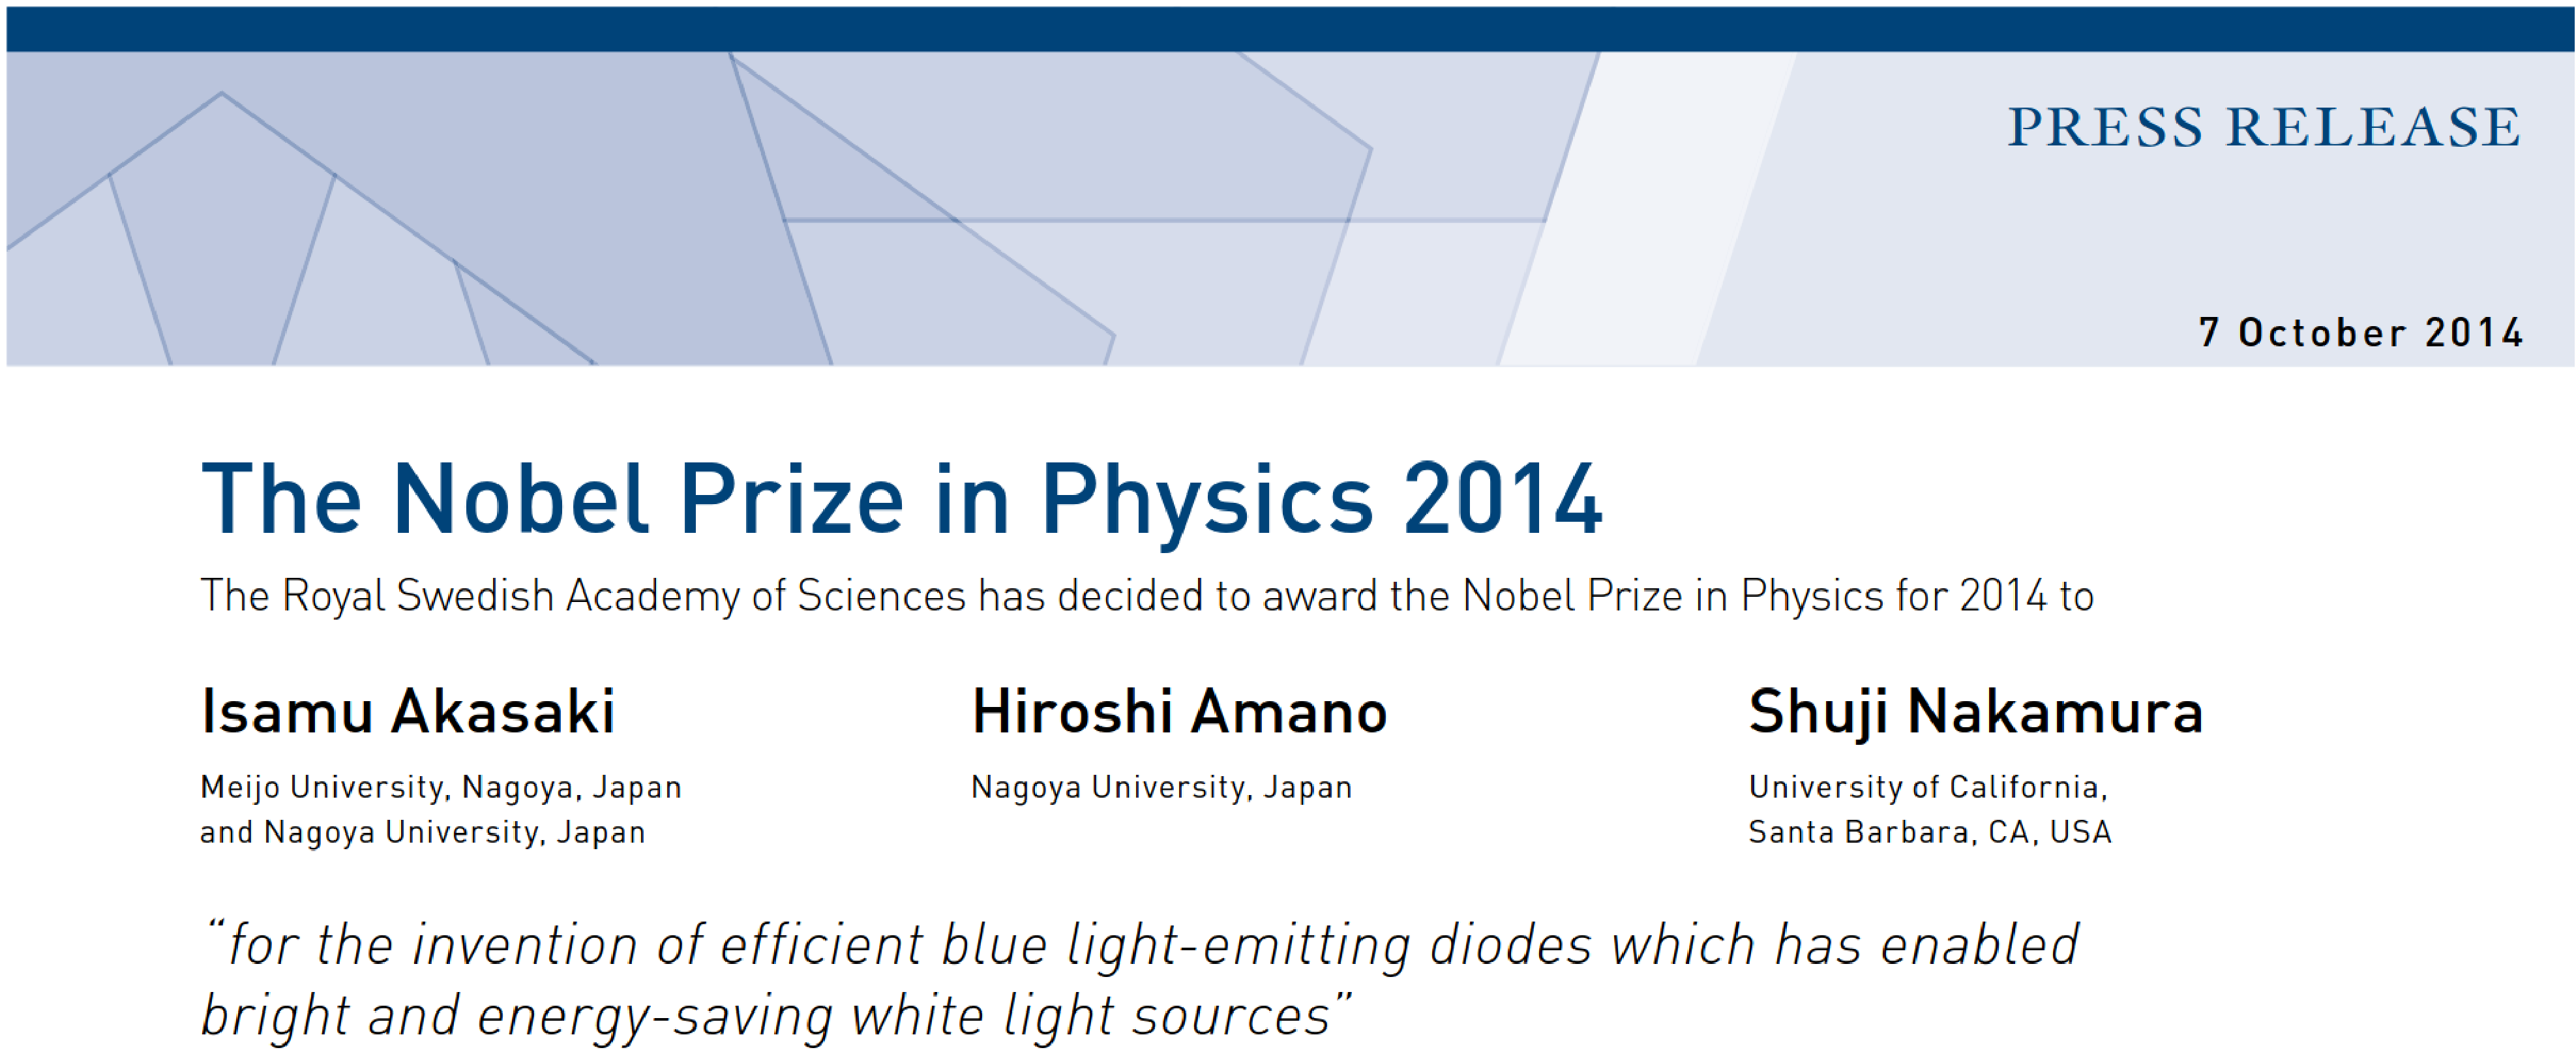
\includegraphics[width=\textwidth]{sep3_images/Nobel.pdf}
  \\~\\
  The Royal Swedish Academy of Sciences(瑞典皇家科学院), \\
  Isamu Akasaki(赤崎勇，2021年4月1日逝世，享年92岁), \\
  Hiroshi Amano(天野浩), Shuji Nakamura(中村修二)
  \\~\\
  图及以下英文文字为诺贝尔奖官网对此次工作的简短介绍。
\end{slide}

\begin{slide}{\url{https://www.nobelprize.org/uploads/2018/06/ljussignal_whitesign.jpg}}
  \centering
  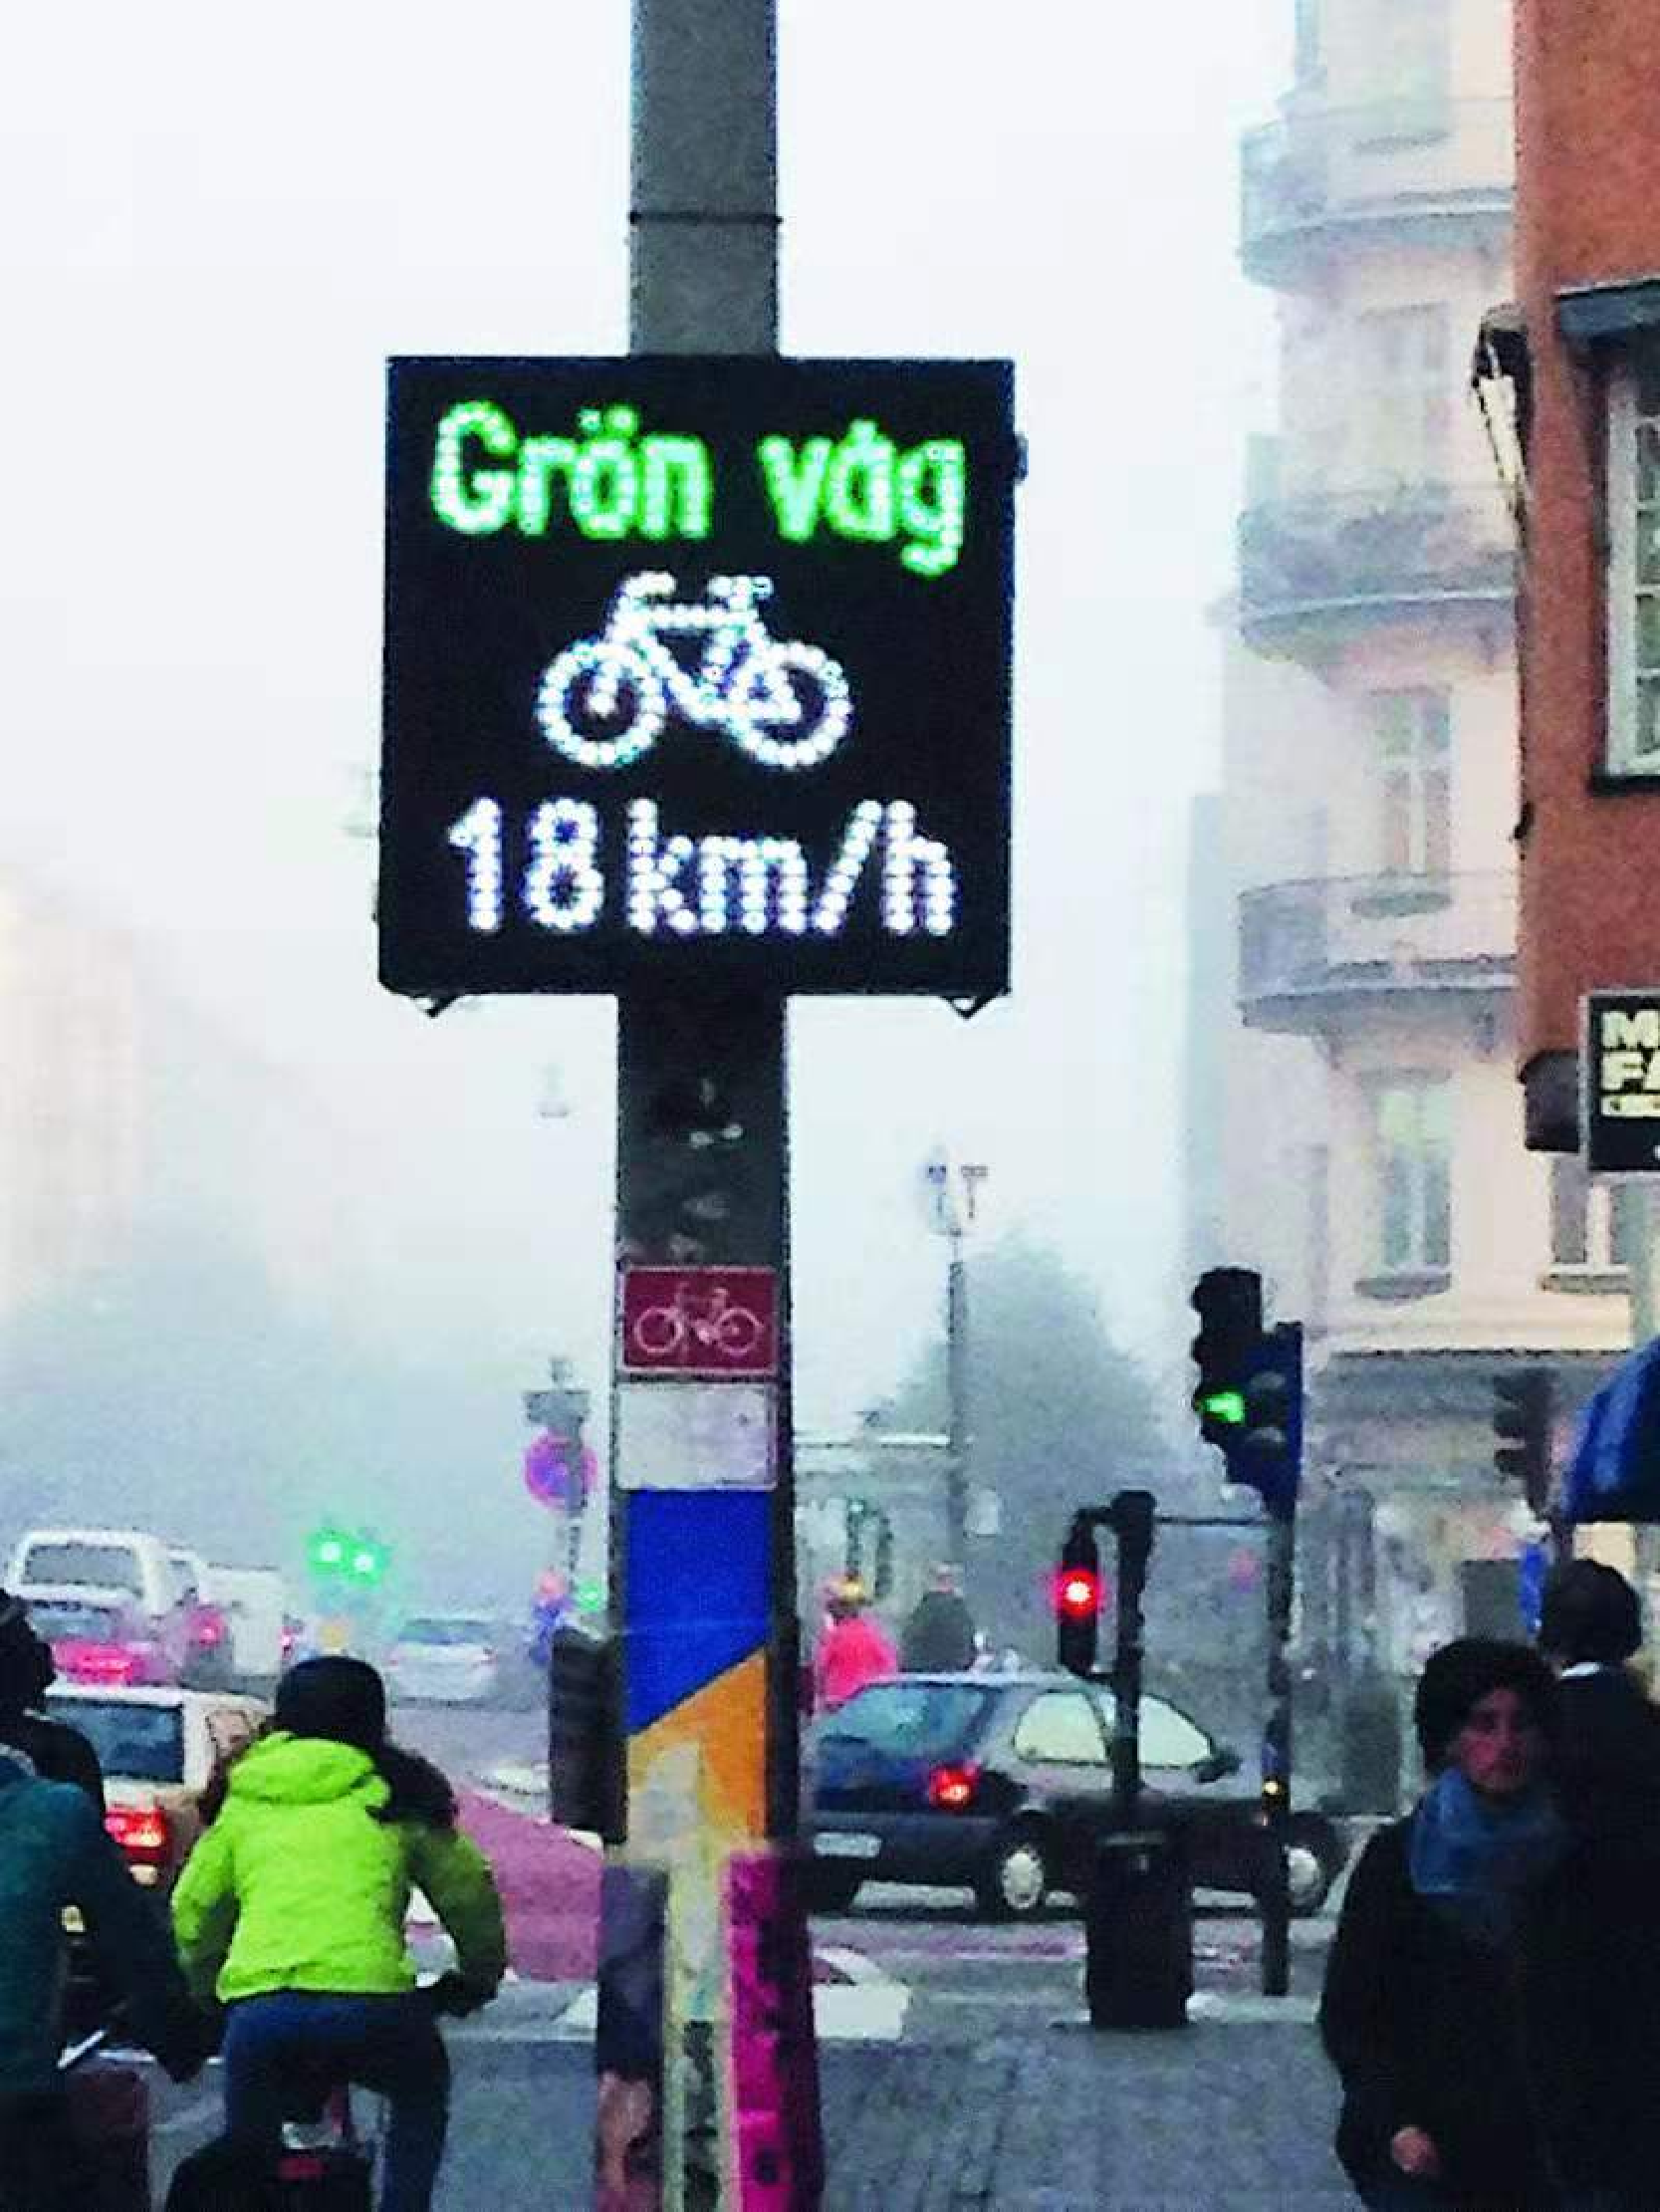
\includegraphics[width=.5\textwidth]{sep3_images/ljussignal_whitesign.pdf}
\end{slide}

\begin{slide}{\url{https://www.nobelprize.org/uploads/2018/06/press-25.pdf}}
  ``When Isamu Akasaki, Hiroshi Amano and Shuji Nakamura produced \textbf{bright blue light beams from their semi-conductors} in the early 1990s, they triggered \textbf{a fundamental transformation of lighting technology}. Red and green diodes had been around for a long time but without blue light, white lamps could not be created. Despite considerable efforts, both in the scientific community and in industry, the blue LED had remained \textbf{a challenge for three decades}.''
  \\~\\
  赤崎勇、天野浩和中村修二在20世纪90年代前期的工作不可不谓之巨大突破。他们使用半导体材料发出了\textbf{明亮的蓝光}，催生了\textbf{发光技术底层的转型}。那时红绿两色的发光二极管已有多年历史，唯有蓝色缺位，白光二极管一直无法制成。此前人们前赴后继\textbf{三十多年}，还是没能解决这个横跨科学界和工业界的\textbf{巨大难题}。
\end{slide}

\begin{slide}{\url{https://www.nobelprize.org/uploads/2018/06/press-25.pdf}}
  ``\textbf{They succeeded where everyone else had failed}. Akasaki worked together with Amano at the University of Nagoya, while Nakamura was employed at Nichia Chemicals, a small company in Tokushima. Their inventions were revolutionary. \textbf{Incandescent light bulbs lit the 20th century; the 21st century will be lit by LED lamps.}''
  \\~\\
  \textbf{他们在万人跌倒之处成功了}！赤崎勇和天野浩一起在名古屋大学工作，而中村修二在日亚化学工业株式会社（日本四国岛东岸港市德岛的一家小公司）工作。他们的发明是革命性的。\textbf{白炽灯照亮了\textbf{20}世纪，而\textbf{21}世纪将为\textbf{LED}灯所点亮。}
\end{slide}

\begin{slide}{\url{https://www.nobelprize.org/uploads/2018/06/press-25.pdf}}
  \small
  ``White LED lamps emit a bright white light, are \textbf{long-lasting and energy-efficient}. They are constantly improved, getting more efficient with higher luminous flux (measured in lumen) per unit electrical input power (measured in watt). The most recent record is \textbf{just over 300 lm/W}, which can be compared to 16 for regular light bulbs and close to 70 for fluorescent lamps. As \textbf{about one fourth of world electricity consumption} is used for lighting purposes, the LEDs contribute to saving the Earth’s resources. Materials consumption is also diminished (减少) as LEDs last \textbf{up to 100,000 hours}, compared to 1,000 for incandescent bulbs and 10,000 hours for fluorescent lights.''
  \\~\\
  白光二极管发光明亮，\textbf{持久，且节能}。它们不断随更新换代而变得越来越高效，即单位输入电功率（单位瓦特）获得的照度（单位流明）不断提高。其流明瓦特比\textbf{最近刚好超过了}\textbf{300 lm/W}，该指标对于常规灯泡而言仅16，荧光灯接近70。由于\textbf{世界上大约四分之一的电都消耗在了照明用途上}，LED为全球节能带来了巨大贡献。由于LED寿命\textbf{长达十万小时}，相比之下白炽灯只有一千小时，荧光灯有一万小时，制造光源所需的材料损耗亦同步减少。
\end{slide}

\begin{slide}{\url{https://www.nobelprize.org/uploads/2018/06/efficiency.pdf}}
  \vspace{1em}\hspace{-.1\textwidth}
  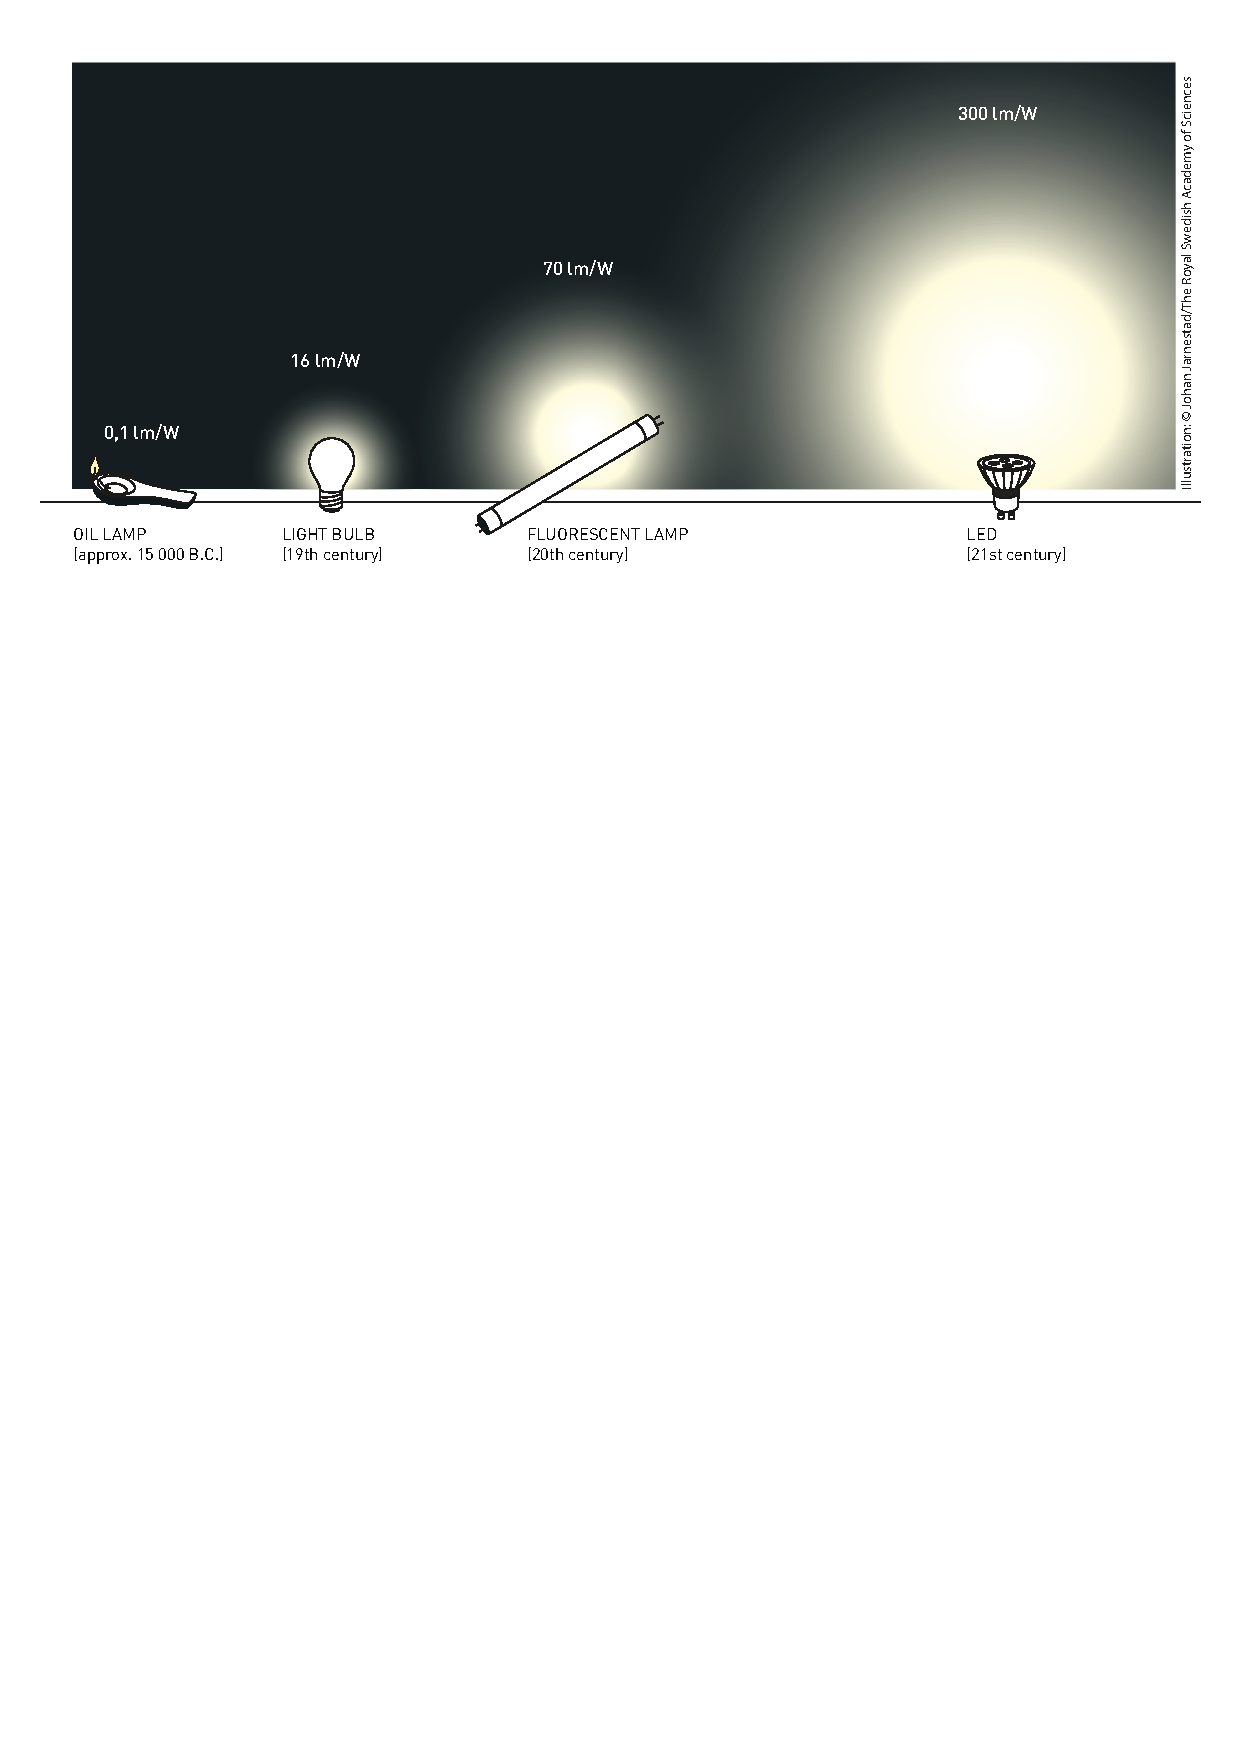
\includegraphics[width=1.2\textwidth]{sep3_images/efficiency.pdf}
\end{slide}

\begin{slide}{\url{https://www.nobelprize.org/uploads/2018/06/press-25.pdf}}
  ``The LED lamp holds great promise for increasing the quality of life for \textbf{over 1.5 billion people} around the world who lack access to electricity grids: due to \textbf{low power requirements} it can be powered by \textbf{cheap local solar power}.''
  \\~\\
  ``The invention of the efficient blue LED is \textbf{just twenty years old}, but it has already contributed to create white light in an entirely new manner to the benefit of us all.''
  \\~\\
  LED灯对提高全球\textbf{超过\textbf{1.5}亿与电网隔绝的人口}的生活质量大有前景：它\textbf{需要的电功率很小}，可以使用\textbf{当地便宜的太阳能}供电。高效蓝光LED的发明利在千秋，这项发明\textbf{不过二十年前}，但已完全革新了人类产生白光的方式。
\end{slide}

\section{发展历史}

\begin{slide}{\url{https://en.wikipedia.org/wiki/Light-emitting_diode}}
  ``The first blue-violet LED using \textbf{magnesium-doped gallium nitride} was made at Stanford University in 1972 by Herb Maruska and Wally Rhines, doctoral students in materials science and engineering. At the time Maruska was on leave from RCA Laboratories, where he collaborated with Jacques Pankove on related work.''
  \\~\\
  发展历史部分主要参考维基百科综述。
  \\~\\
  世界首个蓝紫光LED由美国斯坦福大学于1972年使用\textbf{掺镁氮化镓}制成，主要贡献者为Herb Maruska和Wally Rhines，他们是材料科学与工程专业的博士生。那时Maruska正休假，不在RCA实验室，在那个实验室里他与Jacques Pankove在发光二极管有关工作中合作。
\end{slide}

\begin{slide}{\url{https://en.wikipedia.org/wiki/Light-emitting_diode}}
  ``In 1971, the year after Maruska left for Stanford, his RCA colleagues Pankove and Ed Miller demonstrated \textbf{the first blue electroluminescence from zinc-doped gallium nitride}, though the subsequent device Pankove and Miller built, \textbf{the first actual gallium nitride light-emitting diode, emitted green light}.''
  \\~\\
  1971年，也就是Maruska离开斯坦福大学的一年后，他的RCA同事Pankove和Ed Miller演示了\textbf{首次掺锌氮化镓的蓝色电致发光}，通过Pankove和Miller建造的后续装置，\textbf{首个货真价实的氮化镓LED发出了绿光}。
\end{slide}

\begin{slide}{\url{https://en.wikipedia.org/wiki/Light-emitting_diode}}
  ``In 1974 the U.S. Patent Office awarded Maruska, Rhines and Stanford professor David Stevenson a patent for their work in 1972. Today, \textbf{magnesium-doping of gallium nitride remains the basis for all commercial blue LEDs and laser diodes}. In the early 1970s, these devices were too dim for practical use, and research into gallium nitride devices slowed.''
  \\~\\
  1974年，美国专利局给Maruska、Rhines和斯坦福教授David Stevenson一行人1972年的工作授予了专利。今天，\textbf{掺镁氮化镓仍然是商用蓝光二极管和激光二极管的基础}。20世纪70年代前期，这些设备的实用价值还不清楚，有关氮化镓设备的研究放缓。
\end{slide}

\begin{slide}{\url{https://en.wikipedia.org/wiki/Light-emitting_diode}}
  ``In August 1989, Cree introduced the first commercially available blue LED based on \textbf{the indirect bandgap semiconductor, silicon carbide (SiC)}. SiC LEDs had \textbf{very low efficiency}, no more than about 0.03\%, but \textbf{did emit in the blue portion of the visible light spectrum}.''
  \\~\\
  1989年八月，Cree以\textbf{间接带隙半导体碳化硅}为基础引进了首个商用的蓝光二极管。碳化硅LED\textbf{效率极低}，不超过0.03\%，但它\textbf{真真切切地能在可见光波段发蓝光}。
\end{slide}

\begin{slide}{\url{https://en.wikipedia.org/wiki/Light-emitting_diode}}
  ``In the late 1980s, key breakthroughs in \textbf{GaN epitaxial growth and p-type doping} ushered in the modern era of GaN-based optoelectronic devices. Building upon this foundation, Theodore Moustakas at Boston University patented a method for producing high-brightness blue LEDs using a new two-step process in 1991.''
  \\~\\
  二十世纪80年代后期，\textbf{氮化镓外延生长技术和p型掺杂技术}的关键突破引领了近代以氮化镓为基础的光电设备时代。在此基础上，1991年波士顿大学的Theodore Moustakas获得了使用新型two-step process产生高亮度蓝光二极管方法的专利。
\end{slide}

\begin{slide}{\url{https://en.wikipedia.org/wiki/Light-emitting_diode}}
  ``Two years later, in 1993, \textbf{high-brightness blue LEDs were demonstrated by Shuji Nakamura of Nichia Corporation using a gallium nitride growth process}. In parallel, Isamu Akasaki and Hiroshi Amano of Nagoya University were working on \textbf{developing the important GaN deposition on sapphire substrates and the demonstration of p-type doping of GaN}. This new development revolutionized LED lighting, making high-power blue light sources practical, leading to the development of technologies like Blu-ray.''
  \\~\\
  两年后，也就是1993年，\textbf{高亮蓝光二极管由日本日亚化学工业株式会社的中村修二使用氮化镓生长过程制成}。与此同时，名古屋大学的赤崎勇和天野浩正致力于\textbf{研发氮化镓在蓝宝石衬底上的重要沉积和氮化镓p型掺杂的实现}。这些新进展对LED发光技术带来了革命性影响，使得制造高功率蓝光源变得切实可行，引领了蓝光光碟等技术的发展。
\end{slide}

\begin{slide}{\url{https://en.wikipedia.org/wiki/Light-emitting_diode}}
  ``Nakamura was awarded the 2006 Millennium Technology Prize for his invention. Nakamura, Hiroshi Amano and Isamu Akasaki were awarded the Nobel Prize in Physics in 2014 for the invention of the blue LED. In 2015, a US court ruled that three companies had infringed Moustakas's prior patent, and ordered them to pay licensing fees of not less than US\$13 million.''
  \\~\\
  中村修二因其发明被授予2006年度千禧年科技奖。中村修二、赤崎勇和天野浩因其蓝光二极管的发明被授予2014年度诺贝尔物理学奖。2015年，一美法院裁决三家公司侵犯了Moustakas早先的专利权，责令其支付不少于一千三百万美元的授权费。
\end{slide}

% \begin{slide}
% In 1995, Alberto Barbieri at the Cardiff University Laboratory (GB) investigated the efficiency and reliability of high-brightness LEDs and demonstrated a "transparent contact" LED using indium tin oxide (ITO) on (AlGaInP/GaAs).
% \\~\\
% 1995年，英国卡迪夫大学的Alberto Barbieri调查了高亮二极管的效率和可靠性，使用AlGaInP/GaAs上的氧化铟锡实现了“透明接触”LED。
% \end{slide}
%
% \begin{slide}
% In 2001 and 2002, processes for growing gallium nitride (GaN) LEDs on silicon were successfully demonstrated. In January 2012, Osram demonstrated high-power InGaN LEDs grown on silicon substrates commercially, and GaN-on-silicon LEDs are in production at Plessey Semiconductors.
% \\~\\
% 2001至2002年，硅上的氮化镓LED生长过程成功实现。2012年1月，Osram实现了商用硅基高功率铟镓氮LED生长，硅上氮化镓LED在英国普莱塞半导体公司量产。
% \end{slide}
%
% \begin{slide}
% As of 2017, some manufacturers are using SiC as the substrate for LED production, but sapphire is more common, as it has the most similar properties to that of gallium nitride, reducing the need for patterning the sapphire wafer (patterned wafers are known as epi wafers).
% \\~\\
% 至2017年，一些加工厂使用碳化硅作为LED生产的基底，但蓝宝石使用更为广泛，因其与氮化镓性质最为相似，减少了模式化蓝宝石晶圆的需求（我们知道，模式化的晶圆是外延片）。
% \\~\\
% P.S. 对不起，这里以及后面实在是看不懂了$- \_{} -$
% \end{slide}

% \begin{slide}
% Blue LEDs have an active region consisting of one or more InGaN quantum wells sandwiched between thicker layers of GaN, called cladding layers. By varying the relative In/Ga fraction in the InGaN quantum wells, the light emission can in theory be varied from violet to amber.
% \\~\\
% 蓝光二极管有一个活动区域，包括一个或多个铟镓氮量子势阱，处于更厚层的氮化镓之间，称为包层。由于铟镓氮量子势阱中的相对In/Ga分数不同，理论上其发光分布于紫色到黄褐色。
% \end{slide}
%
% \begin{slide}
% Aluminium gallium nitride (AlGaN) of varying Al/Ga fraction can be used to manufacture the cladding and quantum well layers for ultraviolet LEDs, but these devices have not yet reached the level of efficiency and technological maturity of InGaN/GaN blue/green devices.
% \\~\\
% 不同Al/Ga分数的铝镓氮可用于制作紫外LED的镀层和量子势阱层，但其工艺尚未达到制造InGaN/GaN蓝光或绿光设备一样的高效和技术上成熟之水准。
% \end{slide}

\section{发光原理和技术难点}

\begin{slide}{\url{https://www.nobelprize.org/uploads/2018/06/diode.pdf}}
  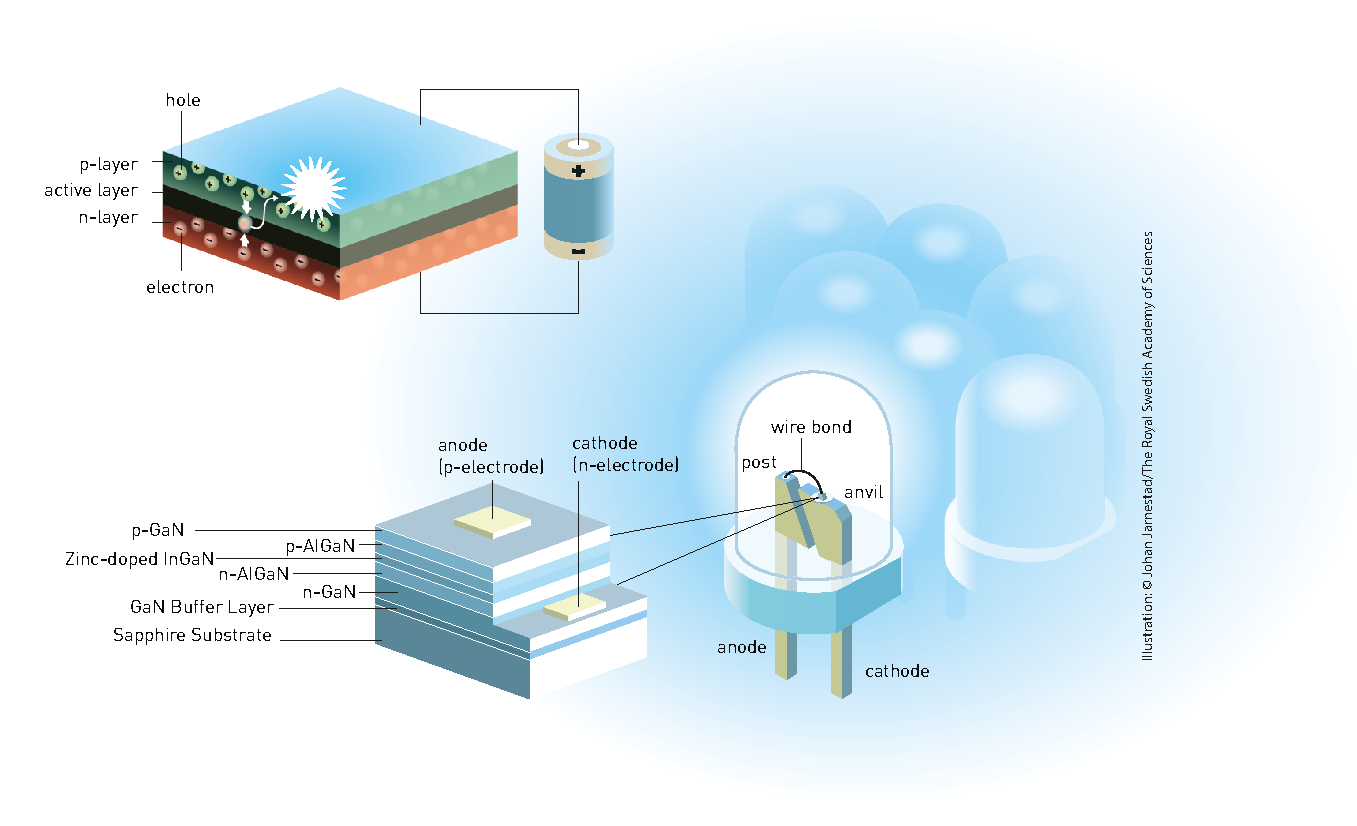
\includegraphics[width=\textwidth]{sep3_images/diode.pdf}
  Sapphire Substrate: 蓝宝石基片
\end{slide}

\begin{slide}{\url{https://www.azom.com/article.aspx?ArticleID=11451}}
  ``On 7th October 2014, Isamu Akasaki, Hiroshi Amano and Shuji Nakamura were awarded the Nobel Prize in Physics for the invention of efficient blue light-emitting diodes (LEDs). Red and green LEDs were created in a number of laboratories during the 1950s and 1960s but it took \textbf{another three decades to finally produce efficient blue LEDs} --- why were they so hard to make?''
  \\~\\
  以下这篇文章介绍了蓝光二极管的结构、发光原理及两项主要的技术困难。其中也穿插了不少科学史。
  \\~\\
  蓝光二极管比红光和绿光二极管的到来晚了三十年，这一诺贝尔奖的工作为何如此困难？
\end{slide}

\begin{slide}{\url{https://www.azom.com/article.aspx?ArticleID=11451}}
  ``Light-emitting diodes are electronic devices which are \textbf{illuminated by the movement of electrons in a semiconductor material}. LEDs are able to emit light with a range of wavelengths from the infrared to the ultraviolet.''
  \\~\\
  ``A semiconductor is a material with an electrical conductivity which is \textbf{somewhere between a conductor such as copper (铜)}, and an \textbf{insulator such as rubber（橡皮）}. They are usually \textbf{made from a poor conductor which is then ‘doped’ by adding atoms of another material to it}.''
  \\~\\
  简单地说，LED发光源于半导体材料中电子的移动（电致发光）。所谓半导体，其导电能力介于导体和绝缘体之间。半导体常由不良导体掺杂制成。所谓掺杂，就是在材料中掺入本不属于该材料组分的其他原子。
\end{slide}

\begin{slide}{\url{https://www.azom.com/article.aspx?ArticleID=11451}}
  ``LEDs are typically made from \textbf{aluminum-gallium-arsenide (AlGaAs)} which in its pure form does not contain any free electrons to conduct electrical current. As a result, AlGaAs is \textbf{doped with either free electrons or ‘electron holes’ in order to change the materials balance and make it more conductive}.''
  \\~\\
  ``What is an \textbf{Electron Hole}? The absence of an electron from an \textbf{otherwise full valence band}.''
  \\~\\
  一般LED用AlGaAs制成，这种材料本身不带有可以导电的自由电子。人们在其中掺杂，使其内部含有自由电子或电子空穴，改变其物料平衡，改善其导电性。所谓电子空穴，即因中心原子的共价键缺失导致的缺电子现象，是一种物理模型，而非真实存在的物理实体。
\end{slide}

\begin{slide}{\url{https://www.azom.com/article.aspx?ArticleID=11451}}
  ``Semiconductors can be classified into two types of material; N-type and P-type:''
  \\~\\
  ``\textbf{N-type} semiconductors contain extra negatively charged \textbf{electrons} and as a result the free electrons flow from negatively charged areas to positively charged areas.''
  \\~\\
  ``\textbf{P-type} semiconductors have \textbf{extra holes which allows free electrons to jump between the holes} and moving from negatively charged areas to positively charged areas as a result.''
  \\~\\
  因掺杂类型的不同，半导体分为N型（negtive）和P型（positive）。N型半导体的载流子为富余电子，P型半导体的载流子为富余空穴。空穴导电并非空穴本身移动，而是电子在不同空穴间跳转，等效地看，就是空穴在向电子运动的反方向移动。
\end{slide}

\begin{slide}{\url{https://www.azom.com/article.aspx?ArticleID=11451}}
  ``A diode consists of a section of an N-type semiconductor attached to a section of a P-type semiconductor (known as a \textbf{p-n junction}) with two electrodes (电极) placed at either end of this arrangement. When current flows across a diode, the negatively charged electrons move in one direction in the material and the positively charged holes move in the opposite direction. As the holes exist in lower energy states, \textbf{a free electron will lose energy when it falls to a hole and emit this energy in the form of a photon of light}.''
  \\~\\
  二极管由P-N结组成。所谓P-N结，即两块结合在一起的不同掺杂类型的半导体。电流通过P-N结时，电子和空穴分别向相反的方向移动。电子与空穴可能发生结合，该过程产生能量，并可能以光子的形式放出，这样便会发光。
\end{slide}

\begin{slide}{\url{https://www.azom.com/article.aspx?ArticleID=11451}}
  ``\textbf{The size of the fall in energy determines the energy the photon has when it is emitted, which in turns determines the colour of the light the diode emits}. An emitted photon with a large amount of energy will have a shorter wavelength than light emitted with a lower amount of energy.''
  \\~\\
  电子空穴结合能决定了结合过程释放的能量，进而决定了可能释放出的光子的能量，从而影响发光的颜色。
\end{slide}

\begin{slide}{\url{https://www.azom.com/article.aspx?ArticleID=11451}}
  ``\textbf{The first diode} which was able to emit \textbf{electrically produced light} was created in 1907 by H.J. Round whilst he was experimenting with a cat's-whisker detector. Round applied a potential difference across a \textbf{silicon carbide (SiC) crystal}. He found that \textbf{the colour of light emitted varied depending on the voltage which was applied across the crystal}.''
  \\~\\
  碳化硅是一种可用于生产半导体发光二极管的材料。早在1907年，这种材料就被用于制造最早的LED。碳化硅晶体的发光颜色与供电电压有关，也可发出蓝光，而现在之所以不用它，如前所述，其发光效率太低了。
\end{slide}

% \begin{slide}{\url{https://www.azom.com/article.aspx?ArticleID=11451}}
%   ``During the 1920s and 1930s, the phenomena of electroluminescence was studied by the Soviet physicist who published several journal articles on the subject.''
%   \\~\\
%   ``In 1947, the electronic transistor was invented at Bell Telephone Laboratories thanks in part to the advancement in understanding of semiconductors and p-n junctions.''
%   \\~\\
%   半导体的研究贯穿20世纪，除电致发光现象外，半导体材料的一个更加重要的应用便是晶体管。
% \end{slide}

% \begin{slide}{\url{https://www.azom.com/article.aspx?ArticleID=11451}}
%   ``Electroluminescence was widely studied in detail during the 1950s by scientists, with J.R. Haynes demonstrating that \textbf{the emission of light from germanium and silicon diodes was due to the interaction of holes and electrons in a p-n junction} in 1956 at Bell Telephone Laboratories.''
%   \\~\\
%   ``In 1956, Shockley, Bardeen and Brattain received a Nobel Prize for their research into semiconductors and the discovery of the transistor effect.''
% \end{slide}

\begin{slide}{\url{https://www.azom.com/article.aspx?ArticleID=11451}}
  ``\textbf{Infrared LEDs were created in 1962 using p-n junctions made from GaAs}. This semiconductor material has a direct bandgap of \textbf{1.4 eV}, which directly corresponds to the wavelength of infrared light. By the end of the 1960s, \textbf{red and green LEDs were being manufactured in different countries using p-n junctions made from GaP}. The development of a blue LED however proved far more difficult to scientists.''
  \\~\\
  另一种半导体材料砷化镓被用于制造红外LED，其直接带隙为1.4 eV，落在红外区。还有一种半导体材料磷化镓，适当掺杂做成二极管可以使其发出红光和绿光。而对蓝光而言，就没有那么容易了。
\end{slide}

\begin{slide}{\url{https://www.azom.com/article.aspx?ArticleID=11451}}
  \begin{multicols}{2}
    \footnotesize
    {\centering
    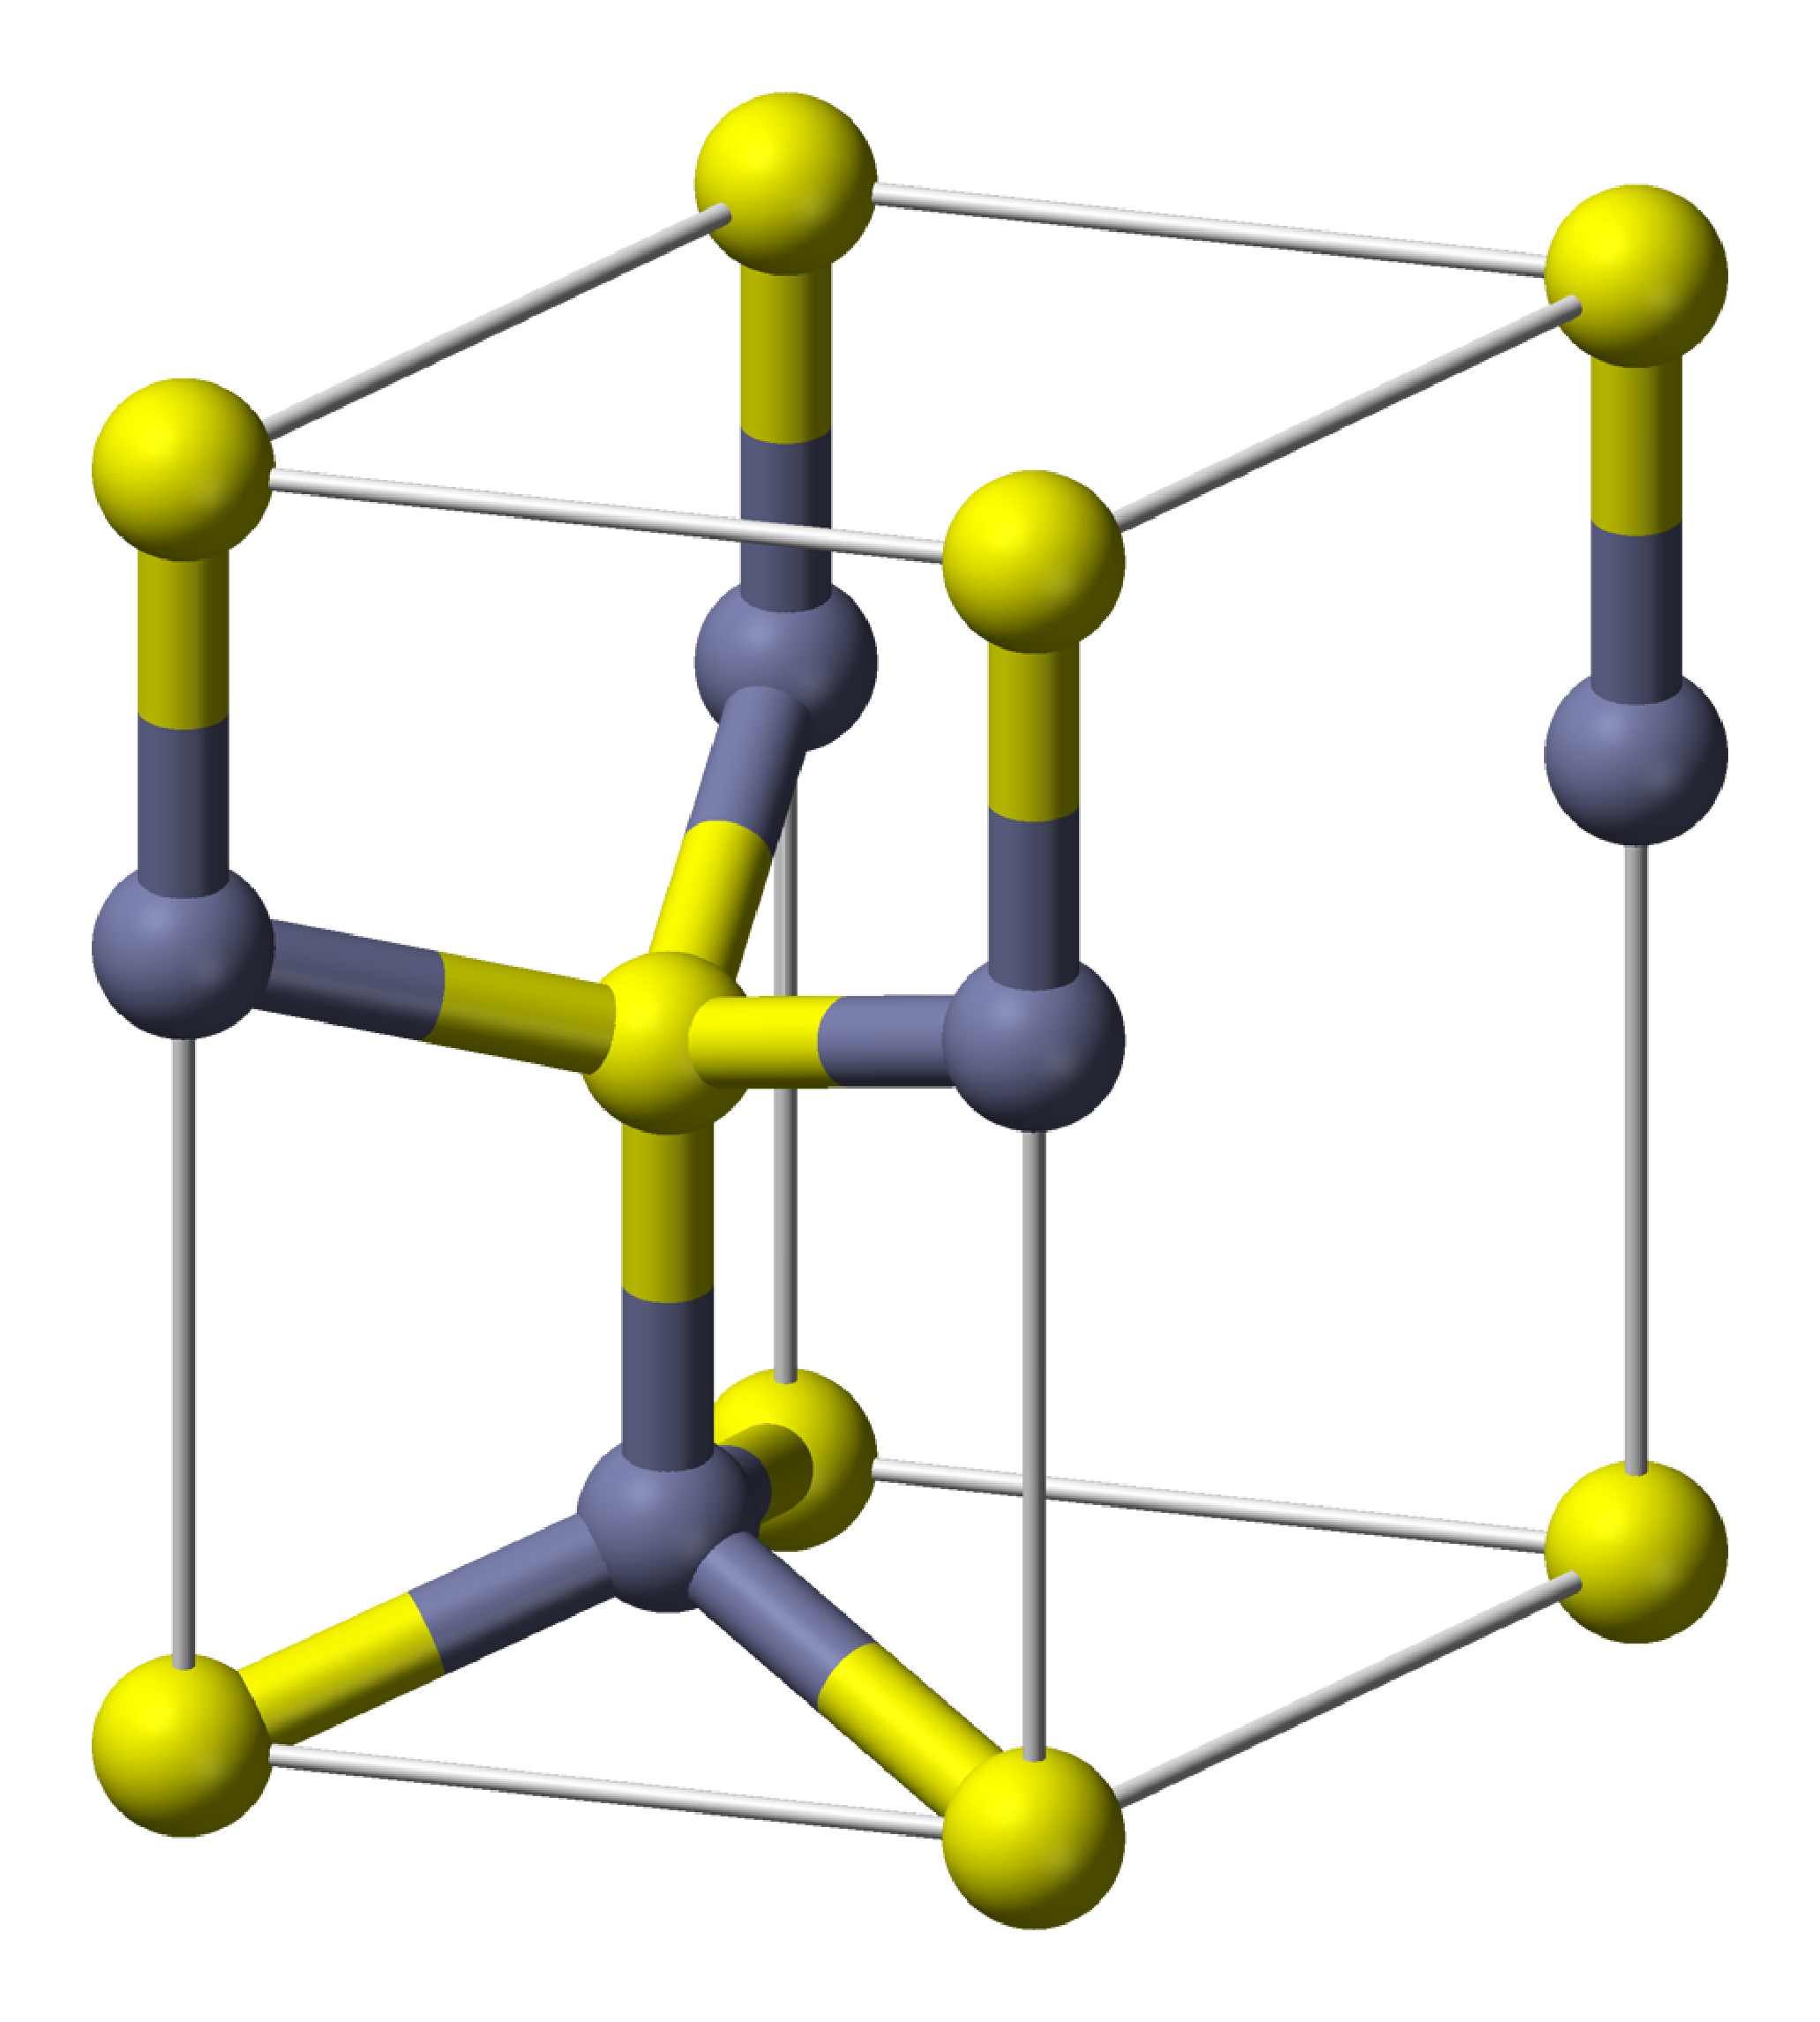
\includegraphics[width=.8\columnwidth]{sep3_images/Wurtzite-unit-cell-3D-balls.pdf} \\
    }
    ``The first attempts at \textbf{the emission of blue light from a diode used ZnSe and SiC}, which are semiconductors with \textbf{high indirect bandgaps, but did not produce efficient light emission}. The material which enabled the development of blue LEDs was \textbf{gallium nitride (GaN)}. GaN is a semiconductor with a Wurtzite（纤锌矿） crystal structure and a \textbf{direct bandgap of 3.4 eV}, which directly corresponds to the wavelength of light in the \textbf{ultraviolet} range.''
    \\~\\
    为了使二极管发蓝光，我们需要寻找高带隙半导体。最先应用的硒化锌和碳化硅制造出的LED发光效率太低。高效的蓝光LED始于氮化镓，其直接带隙3.4 eV，在紫外区。
  \end{multicols}
  {\tiny 图片来源：\url{https://en.wikipedia.org/wiki/File:Wurtzite-unit-cell-3D-balls.png} \\~\\}
\end{slide}

\begin{slide}{\url{https://www.azom.com/article.aspx?ArticleID=11451}}
  ``\textbf{At the end of the 1950s}, researchers at Philips Research Laboratories had considered using GaN to create blue LEDs but instead chose to \textbf{concentrate on devices made from GaP instead due to difficulties in growing GaN crystals}. These crystals were \textbf{more effectively produced in the late 1960s by using the Hydride Vapour Phase Epitaxy (HVPE, 氢化物气相外延) growing GaN on a substrate}.''
  \\~\\
  早在20世纪50年代末，氮化镓便被考虑用于制作蓝光LED，但由于其晶体生长过于困难，飞利浦实验室选择了磷化镓。直至20世纪60年代后期，氮化镓得以高效生产——利用氢化物气相外延法在基片上生长氮化镓晶体。
\end{slide}

\begin{slide}{\url{https://www.azom.com/article.aspx?ArticleID=11451}}
  ``In 1974 Isamu Akasaki began studying gallium nitride and took up a professorship at Nagoya University to continue his research alongside Hiroshi Amano. In 1986 the MOVPE (金属有机物气相外延) technique was used in order to \textbf{produce GaN with high crystal quality and good optical properties}. Shuji Nakamura later development a similar method in order to grown GaN at low temperatures.''
  \\~\\
  可以推断，虽然氮化镓晶体生长在工业上已经实现，其技术水平尚不满足蓝光二极管的制作需求（不然为什么又折腾了三十年）。1974年开始，2014年诺贝尔物理学奖得主们赤崎勇和天野浩开始研究之。1986年，金属有机物气相外延法的出现大大改善了该半导体材料的光学特性。另一位得奖者中村修二随后以低温方法实现了相似技术（可以推断，该技术对于生产蓝光二极管更为高效）。
\end{slide}

\begin{slide}{\url{https://www.azom.com/article.aspx?ArticleID=11451}}
  ``Another major problem in producing blue LEDs was \textbf{the difficulty in p-doping GaN with precision}. In the late 1980s, Amano and Akasaki discovered that \textbf{when GaN was doped with zinc atoms, it emitted more light} and thus this gave better p-doping. This phenomena was later explained in an article by Nakamura. This was an important discovery as it \textbf{paved the way for p-n junctions to be used in gallium nitride semiconductors}.''
  \\~\\
  除氮化镓晶体生长技术外，蓝光二极管生产的另一技术难题是精确p型掺杂问题。该掺杂技术于20世纪80年代后期取得突破，氮化镓掺锌会发更多光，从而更有利于p型掺杂（为什么？）。这一突破为氮化镓材料在蓝光二极管的应用奠定了基础。
\end{slide}

\begin{slide}{\url{https://www.azom.com/article.aspx?ArticleID=11451}}
  ``A \textbf{key step} in the development of blue LEDs was the development of heterojunctions (异质结) in the early 1990s by research groups led by Akasaki and Nakamura.  \textbf{In 1994, Nakamura used a double heterojunction InGaN/AlGaN to produce a device with a quantum efficiency of 2.7\%, which opened the door for efficient blue LEDs to be easily produced}.''
  \\~\\
  蓝光二极管发展成熟的关键一步是异质结的应用。这一重大突破产生于20世纪90年代前期，由二位诺贝尔奖得主赤崎勇和中村修二所贡献。1994年，中村修二使用了双异质结InGaN/AlGaN来制作蓝光LED，其量子效率（是什么意思？）达到了2.7\%，开创了蓝光LED量产的新时代。
\end{slide}

\begin{slide}{\url{https://www.nobelprize.org/uploads/2018/06/diode.pdf}}
  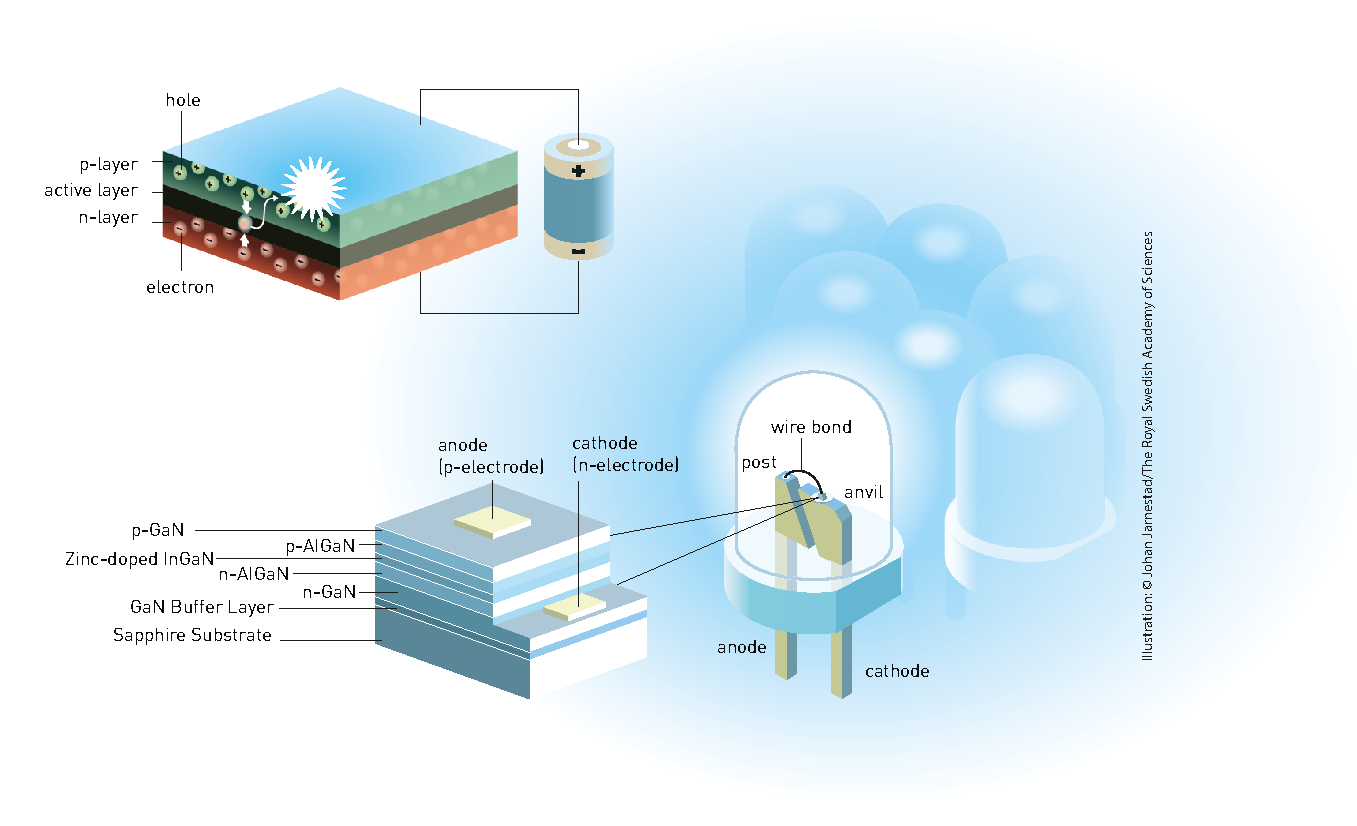
\includegraphics[width=\textwidth]{sep3_images/diode.pdf}
  Sapphire Substrate: 蓝宝石基片
\end{slide}

\begin{slide}{\url{https://www.azom.com/article.aspx?ArticleID=11451}}
  ``\textbf{The emission of blue light based on GaN was observed between 1995 and 1996 by both research groups}. Modern efficient GaN based LEDs are the result of long series of breakthroughs in the scientific fields of materials physics, optics, electronics and chemistry.''
  \\~\\
  终于终于，实验者们在1995年和1996年分别使氮化镓二极管发出了蓝光！同时，如今蓝光二极管的高效离不开长期材料物理、光学、电子学和化学领域的一系列重大突破。
\end{slide}

\begin{slide}{\url{https://www.chemeurope.com/en/news/151134/}}
  ``Scientists at UCL, in collaboration with groups at the University of Bath and the Daresbury Laboratory, have uncovered the mystery of why blue light-emitting diodes (LEDs) are so difficult to make, by revealing \textbf{the complex properties of their main component - gallium nitride} - using sophisticated computer simulations.''
  \\~\\
  下面通过一篇PRL文献的工作介绍看看生产掺杂氮化镓晶体材料的困难。该文献利用复杂的计算机模拟方法，描绘了向氮化镓晶体中掺入镁原子时晶体发生的复杂变化，揭示了掺杂技术的难点所在。
\end{slide}

% \begin{slide}{\url{https://www.chemeurope.com/en/news/151134/}}
%   ``Blue LEDs were first commercialised two decades ago and have been instrumental in the development of new forms of energy saving lighting, earning their inventors the 2014 Nobel Prize in Physics. Light emitting diodes are \textbf{made of two layers of semicon-ducting materials} (insulating materials which can be made conduct electricity in special circumstances). \textbf{One has mobile negative charges, or electrons}, available for conduction, and \textbf{the other positive charges, or holes}. \textbf{When a voltage is applied, an electron and a hole can meet at the junction between the two, and a photon (light particle) is emitted.}''
% \end{slide}

% \begin{slide}{\url{https://www.chemeurope.com/en/news/151134/}}
%   ``The desired properties of a semiconductor layer are achieved by \textbf{growing a crystalline film (结晶膜)} of a particular material and \textbf{adding small quantities of an `impurity' element}, which has more or fewer electrons taking part in the chemical bonding (a process known as \textbf{`doping'}). Depending on the number of electrons, these impurities donate an extra positive or negative mobile charge to the material.''
% \end{slide}

\begin{slide}{\url{https://www.chemeurope.com/en/news/151134/}}
  ``The key ingredient (成分) for blue LEDs is \textbf{gallium nitride, a robust material with a large energy separation, or `gap', between electrons and holes - this gap is crucial in tuning the energy of the emitted photons to produce blue light}. But while doping to donate mobile negative charges in the substance proved to be easy, \textbf{donating positive charges failed completely}. The breakthrough, which won the Nobel Prize, \textbf{required doping it with surprisingly large amounts of magnesium}.''
  \\~\\
  刚才我们提到的获得诺贝尔奖的工作，即双异质半导体蓝光二极管的发明，离不开掺杂技术的突破。刚才我们也提到，p型掺杂是一大技术难题。我们需要在氮化镓晶体中大量地掺入镁原子，让我们来看看这是为什么。
\end{slide}

\begin{slide}{\url{https://www.chemeurope.com/en/news/151134/}}
  {\small ```While blue LEDs have now been manufactured for over a decade,' says John Buckeridge (UCL Chemistry), lead author of the study, `there has always been a gap in our understanding of how they actually work, and this is where our study comes in. Naively, based on what is seen in other common semiconductors such as silicon, you would expect each magnesium atom added to the crystal to donate one hole. But in fact, \textbf{to donate a single mobile hole in gallium nitride, at least a hundred atoms of magnesium have to be added}. It's technically extremely difficult to manufacture gallium nitride crystals with so much magnesium in them, not to mention that it's been frustrating (令人懊恼的) for scientists not to understand what the problem was.'{''}}
  \\~\\
  出乎意料地，模拟实验表明，为了在氮化镓晶体中产生一个正电荷，需要掺入上百的镁原子。掺杂如此之多，在工业上是个困难。然而，其缘由无人能解。
\end{slide}

\begin{slide}
  \begin{multicols}{2}
    \parbox{\columnwidth}{
      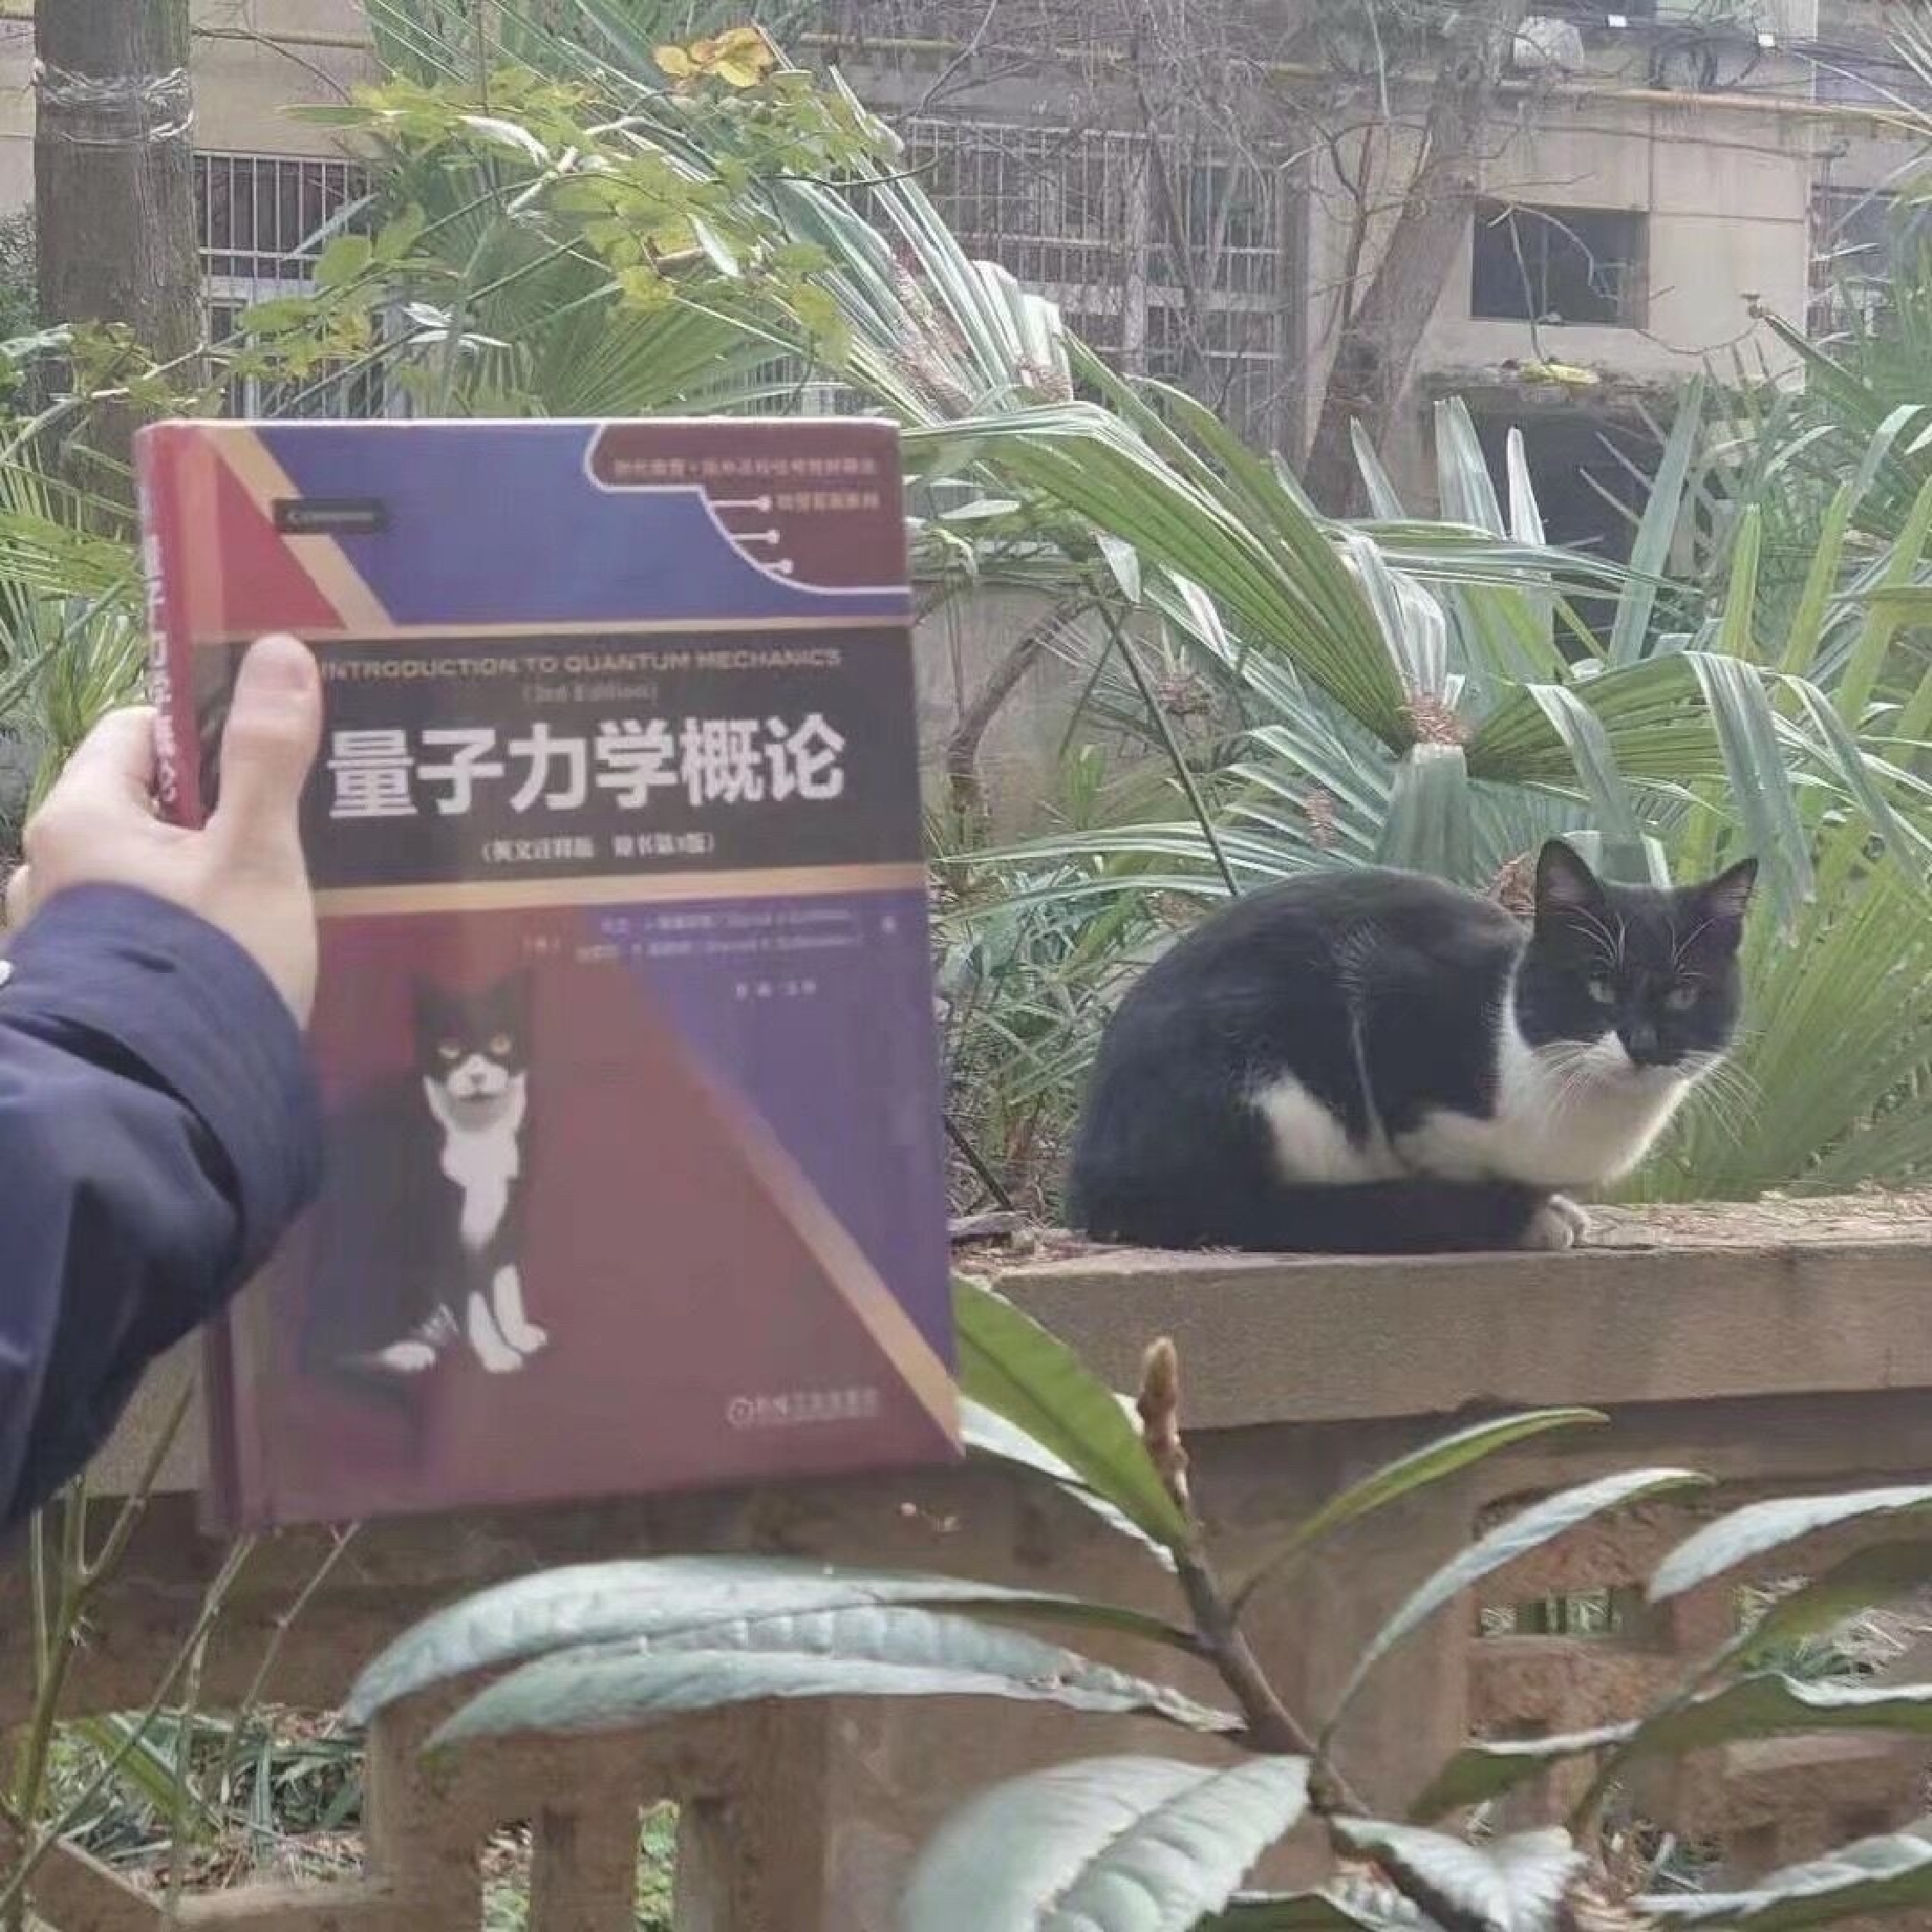
\includegraphics[width=\columnwidth]{sep3_images/cat.pdf} \\
      \tiny 图片来源: \url{https://pkuhelper.pku.edu.cn/hole}
    }
    \kaishu
    \raggedright\qquad 我可以有把握地说，没人懂得量子力学。 \\
    \raggedleft ——理查德·费曼 \\
    ~\\
    \raggedright\qquad 量子力学绝对是上个世纪最伟大的发现，没有之一。没人能弄懂量子力学，但所有这些半导体元件都是量子力学创造出来的。看看，我们的手机，我们的电脑，里面有多少三极管。 \\
    \raggedleft ——赵建业（学生回忆版） \\
  \end{multicols}
\end{slide}

% \begin{slide}{\url{https://www.chemeurope.com/en/news/151134/}}
%   ``The team's study, published today in the journal \textit{Physical Review Letters}, unveils the root of the problem by \textbf{examining the unusual behaviour of doped gallium nitride at the atomic level using highly sophisticated computer simulations}.''
% \end{slide}

\begin{slide}{\url{https://www.chemeurope.com/en/news/151134/}}
  {\small ```To make an accurate simulation of a defect (缺陷) in a semiconductor such as an impurity, we need the accuracy you get from a quantum mechanical model,' explains David Scanlon (UCL Chemistry), a co-author of the paper. `Such models have been widely applied to the study of perfect crystals, where a small group of atoms form a repeating pattern. \textbf{Introducing a defect that breaks the pattern presents a conundrum (难题), which required the UK's largest supercomputer to solve.} Indeed, \textbf{calculations on very large numbers of atoms were therefore necessary but would be prohibitively expensive to treat the system on a purely quantum-mechanical level}.'{''}}
  \\~\\
  如何进行模拟计算呢？纯量子模型本适用于理想晶体，然而掺杂的引入破坏了系统的对称性，如果使用纯量子力学模型，计算量在英国顶级超算级别。实际上，在计算机科学中，这几乎是一个不可解问题，太多的原子需要参与计算了。
\end{slide}

\begin{slide}{\url{https://www.chemeurope.com/en/news/151134/}}
  ``The team's solution was to apply an approach pioneered in another piece of Nobel Prize winning research: \textbf{hybrid quantum and molecular modelling, the subject of 2013's Nobel Prize in Chemistry}. In these models, different parts of a complex chemical system are simulated with different levels of theory.''
  \\~\\
  必须更换模型！团队使用了获得2013年诺贝尔化学奖的主要工作——混合量子分子模型，该模型使得复杂化学系统的计算模拟成为可解问题。该模型使用不同层次的理论模拟复杂化学系统的不同部分，从而大大降低了计算量。
\end{slide}

\begin{slide}{\url{https://www.chemeurope.com/en/news/151134/}}
  \small
  ```The simulation tells us that when you \textbf{add a magnesium atom}, it replaces a gallium atom but \textbf{does not donate the positive charge to the material}, instead keeping it to itself,' says Richard Catlow (UCL Chemistry), one of the study's co-authors. `In fact, to provide enough energy to \textbf{release the charge} will require heating the material \textbf{beyond its melting point}. Even if it were released, it \textbf{would knock an atom of nitrogen out of the crystal, and get trapped anyway in the resulting vacancy}. Our simulation shows that the behaviour of the semiconductor is \textbf{much more complex than previously imagined, and finally explains why we need so much magnesium to make blue LEDs successfully}.'{''}
  \\~\\
  每掺入一个镁原子，将替换掉晶体中的一个镓管子，但可能并不会贡献一个正电荷，相反地，镁原子自己保留了正电荷。想要释放这一正电荷，靠热运动是不可能的，电离能的大小超过了熔点下的热能。即使正电荷释放出来，也可能经历一定的过程挤出一个氮原子并将电荷束缚于氮原子留下的空隙中。模拟表明，半导体行为的复杂程度远超我们想象，镁原子的如此“浪费”解释了需要大量掺杂的原因。
\end{slide}

\begin{slide}{\url{https://www.chemeurope.com/en/news/151134/}}
  ``The simulations crucially fit a complete set of previously unexplained experimental results involving the behaviour of gallium nitride. Aron Walsh (Bath Chemistry) says `We are now \textbf{looking forward to the investigations into heavily defective GaN, and alternative doping strategies to improve the efficiency of solid-state lighting}'.''
  \\~\\
  模拟结果很好地解释了氮化镓掺杂实验中观察到的镁原子“浪费”现象，下一步应当深入研究重掺杂氮化镓以及其他备选的掺杂策略以改进固态照明效率。
\end{slide}

\begin{slide}{技术难点小结}
  \begin{itemize}
    \item 难题之零为找到合适的半导体材料——氮化镓等
    \item 难题之一为特定理化性质的氮化镓等晶体层的制备
    \item 难题之二为氮化镓等半导体材料n型重掺杂的工业实现
    \item 难题之零随时代发展和技术进步迎刃而解，当今氮化镓等材料的广泛应用是难题一二求解的必然结果
    \item 难题之一困扰人类三十年之久，经过几代科学家和技术人员的努力，最终由中村修二等人解决
    \item 难题之二与难题之一相伴而生，在三人掺锌和使用双异质结等新思路下，n型掺杂效率问题得以解决
  \end{itemize}
\end{slide}

\begin{slide}{\url{https://www.nobelprize.org/uploads/2018/06/diode.pdf}}
  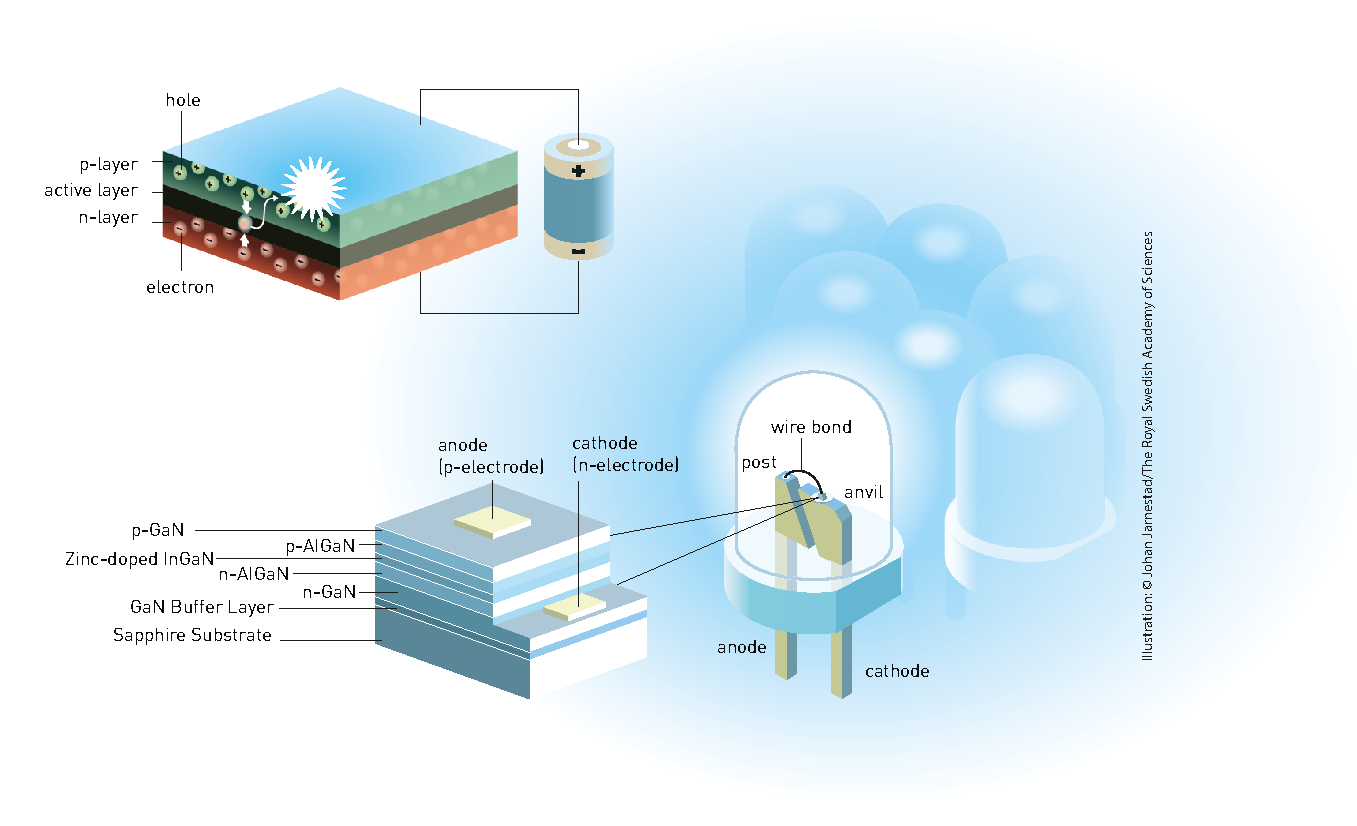
\includegraphics[width=\textwidth]{sep3_images/diode.pdf}
  Sapphire Substrate: 蓝宝石基片
\end{slide}
